% This is the Reed College LaTeX thesis template. Most of the work
% for the document class was done by Sam Noble (SN), as well as this
% template. Later comments etc. by Ben Salzberg (BTS). Additional
% restructuring and APA support by Jess Youngberg (JY).
% Your comments and suggestions are more than welcome; please email
% them to cus@reed.edu
%
% See http://web.reed.edu/cis/help/latex.html for help. There are a
% great bunch of help pages there, with notes on
% getting started, bibtex, etc. Go there and read it if you're not
% already familiar with LaTeX.
%
% Any line that starts with a percent symbol is a comment.
% They won't show up in the document, and are useful for notes
% to yourself and explaining commands.
% Commenting also removes a line from the document;
% very handy for troubleshooting problems. -BTS

% As far as I know, this follows the requirements laid out in
% the 2002-2003 Senior Handbook. Ask a librarian to check the
% document before binding. -SN

%%
%% Preamble
%%
% \documentclass{<something>} must begin each LaTeX document
\documentclass[12pt,twoside]{reedthesis}
% Packages are extensions to the basic LaTeX functions. Whatever you
% want to typeset, there is probably a package out there for it.
% Chemistry (chemtex), screenplays, you name it.
% Check out CTAN to see: http://www.ctan.org/
%%
\usepackage{graphicx,latexsym}
\usepackage{amsmath}
\usepackage{amssymb,amsthm}
\usepackage{longtable,booktabs,setspace}
\usepackage{chemarr} %% Useful for one reaction arrow, useless if you're not a chem major
\usepackage[hyphens]{url}
% Added by CII
\usepackage{hyperref}
\usepackage{lmodern}
\usepackage{float}
\floatplacement{figure}{H}
% End of CII addition
\usepackage{rotating}

% Next line commented out by CII
%%% \usepackage{natbib}
% Comment out the natbib line above and uncomment the following two lines to use the new
% biblatex-chicago style, for Chicago A. Also make some changes at the end where the
% bibliography is included.
%\usepackage{biblatex-chicago}
%\bibliography{thesis}


% Added by CII (Thanks, Hadley!)
% Use ref for internal links
\renewcommand{\hyperref}[2][???]{\autoref{#1}}
\def\chapterautorefname{Chapter}
\def\sectionautorefname{Section}
\def\subsectionautorefname{Subsection}
% End of CII addition

% Added by CII
\usepackage{caption}
\captionsetup{width=5in}
% End of CII addition

% \usepackage{times} % other fonts are available like times, bookman, charter, palatino

% Syntax highlighting #22

% To pass between YAML and LaTeX the dollar signs are added by CII
\title{Pronouns Good or Bad: Attitudes and Relationships with Gendered Pronouns in Gender-Diverse Undergraduates}
\author{Jade Fung}
% The month and year that you submit your FINAL draft TO THE LIBRARY (May or December)
\date{May 2020}
\division{Philosophy, Religion, Psychology, and Linguistics}
\advisor{Vasiliy Safin}
\institution{Reed College}
\degree{Bachelor of Arts}
%If you have two advisors for some reason, you can use the following
% Uncommented out by CII
% End of CII addition

%%% Remember to use the correct department!
\department{Psychology}
% if you're writing a thesis in an interdisciplinary major,
% uncomment the line below and change the text as appropriate.
% check the Senior Handbook if unsure.
%\thedivisionof{The Established Interdisciplinary Committee for}
% if you want the approval page to say "Approved for the Committee",
% uncomment the next line
%\approvedforthe{Committee}

% Added by CII
%%% Copied from knitr
%% maxwidth is the original width if it's less than linewidth
%% otherwise use linewidth (to make sure the graphics do not exceed the margin)
\makeatletter
\def\maxwidth{ %
  \ifdim\Gin@nat@width>\linewidth
    \linewidth
  \else
    \Gin@nat@width
  \fi
}
\makeatother

%Added by @MyKo101, code provided by @GerbrichFerdinands
\newlength{\cslhangindent}
\setlength{\cslhangindent}{1.5em}
\newenvironment{cslreferences}%
  {\setlength{\parindent}{0pt}%
  \everypar{\setlength{\hangindent}{\cslhangindent}}\ignorespaces}%
  {\par}

\renewcommand{\contentsname}{Table of Contents}
% End of CII addition

\setlength{\parskip}{0pt}

% Added by CII

\providecommand{\tightlist}{%
  \setlength{\itemsep}{0pt}\setlength{\parskip}{0pt}}

\Acknowledgements{

}

\Dedication{

}

\Preface{

}

\Abstract{

}

	\usepackage{booktabs}
 \usepackage{longtable}
 \usepackage{array}
 \usepackage{multirow}
 \usepackage{wrapfig}
 \usepackage{float}
 \usepackage{colortbl}
 \usepackage{pdflscape}
 \usepackage{tabu}
 \usepackage{threeparttable}
 \usepackage{threeparttablex}
 \usepackage[normalem]{ulem}
 \usepackage{makecell}
 \usepackage{xcolor}
% End of CII addition
%%
%% End Preamble
%%
%
\begin{document}

% Everything below added by CII
  \maketitle

\frontmatter % this stuff will be roman-numbered
\pagestyle{empty} % this removes page numbers from the frontmatter



  \hypersetup{linkcolor=black}
  \setcounter{tocdepth}{2}
  \tableofcontents

  \listoftables

  \listoffigures



\mainmatter % here the regular arabic numbering starts
\pagestyle{fancyplain} % turns page numbering back on

\hypertarget{introduction}{%
\chapter*{Introduction}\label{introduction}}
\addcontentsline{toc}{chapter}{Introduction}

My introduction bit will go here :-)

\hypertarget{literature-review}{%
\chapter{Literature Review}\label{literature-review}}

Let's review: gendered pronouns.

\hypertarget{methods}{%
\chapter{Methods}\label{methods}}

\hypertarget{participants}{%
\section{Participants}\label{participants}}

477 undergraduate students from Reed College in Portland, Oregon participated in an online survey about ``attitudes towards gendered pronouns.'' Participants were recruited through online advertisements and posters around campus. Notably, this sample is around one-third of the undergraduate student body. Data collection was conducted over a two month period, starting in February 2020. It should also be noted that the global pandemic that occurred in early 2020 shortened our opportunity to collect data.

Participants of all genders were recruited, including cisgender participants. Tate, Youssef, \& Bettergarcia (2014) advocate for the integration of cisgender and non-cisgender gender research into one body of research on gender identity development. They push back on the common assumption that cisgender people do not undergo a period of self-reflection and self-categorization in the maturation of their gender identity. Furthermore, by not excluding cisgender participants from the study, we allowed freer self-categorization e.g.~for the inclusion of people who identified as cisgender and non-binary.

\hypertarget{transgender-inclusive-behavior-scale-tibs}{%
\section{Transgender Inclusive Behavior Scale (TIBS)}\label{transgender-inclusive-behavior-scale-tibs}}

The Transgender Inclusive Behavior Scale was developed by Kattari, O'Connor, \& Kattari (2018) to provide a measure for actions and modes of communication that are inclusive and supportive of transgender people. The TIBS was developed for participants of all gender identities---not exclusively cisgender people.

The TIBS includes a broad array of trans affirming behaviors. This includes several items such as sharing their own pronouns and asking for others', educating themselves on local policies that may affect transgender people, and speaking out against transphobia in their communities.

Responses were collected as five-point likert scales ranging from ``Never'' to ``Always.'' Each participant's responses were added to produce a score that generally represented how many inclusive behaviors one performed.

While selecting our measures, we elected to use the TIBS in lieu of a measure such as the transphobia scale developed by Nagoshi et al. (2008). This was done to generally frame the study as positive and affirming for transgender people. Administering questions about transphobic attitudes to transgender people who are the victims of transphobia and transmisogynistic violence could have been significantly more distressing than asking about affirming and supportive behaviors. Essentially, the TIBS was included as a proxy for how intentionally participants supported and affirmed their transgender peers.

An added potential benefit to administering the TIBS to cisgender participants is that it potentially includes actions that cisgender people had not yet considered doing to support their transgender peers. As data collection progressed, the author received several messages from participants reporting that they had never considered some of the actions, like ensuring that gender-neutral bathrooms were available at events that they organized.

\hypertarget{transgender-congruence-scale-tcs}{%
\section{Transgender Congruence Scale (TCS)}\label{transgender-congruence-scale-tcs}}

The Transgender Congruence Scale was developed by Kozee, Tylka, \& Bauerband (2012) to provide a measure for how transgender people feel ``genuine, authentic, and comfortable with their gender identity and external appearance.'' The TCS was developed for transgender participants. However, we elected to administer the TCS to cisgender participants as well. This was done to avoid presuming that cisgender people have a purely passive relationship with their gender, as is advocated for by Tate et al. (2014).

Responses were collected as five-point likert scales ranging from ``Strongly Disagree'' to ``Strongly Agree'' Each participant's responses were added to produce a score that generally represented how congruent one felt with one's gender identity. The TCS consists of 12 items that include relationships between the participant's gender identity, their physical appearance and presentation, their body, and their social experience with gender.

\hypertarget{gendered-pronoun-attitude-survey-gpas}{%
\section{Gendered Pronoun Attitude Survey (GPAS)}\label{gendered-pronoun-attitude-survey-gpas}}

The GPAS was developed as a broad survey of undergraduate students' relationships and experiences with gendered pronouns. Many items were phrased similarly to questions from the TCS. However, as this is a very novel area of study, the author created most of them herself in consultation with other gender-diverse peers.

Responses were collected as five-point likert scales ranging from ``Strongly Disagree'' to ``Strongly Agree.'' In the first block of questions, participants were asked to report their experiences from the past two weeks. This was done to reflect the Transgender Congruence Scale (TCS) by Kozee et al. (2012). The TCS asked participants to reflect on their relationship with gender in the past two weeks.
\begin{table}

\caption{\label{tab:unnamed-chunk-1}Pronoun attitude questionnaire items: past 2 weeks}
\centering
\begin{tabular}[t]{l}
\hline
Item Description\\
\hline
I feel comfortable sharing my pronouns in most settings.\\
\hline
I feel comfortable sharing my pronouns in non-academic settings in the Reed community.\\
\hline
I feel comfortable sharing my pronouns in classes at Reed.\\
\hline
I want to share my pronouns in most settings.\\
\hline
I want to share my pronouns in non- academic settings in the Reed community.\\
\hline
I want to share my pronouns in classes at Reed.\\
\hline
I feel more comfortable sharing my pronouns if I am with people who may have similar gender identities to me.\\
\hline
I feel more comfortable introducing myself with my pronouns if someone else does first.\\
\hline
I feel more comfortable introducing myself with my pronouns in class if the professor does first.\\
\hline
I am concerned that sharing my pronouns will draw unwanted attention to myself in most settings.\\
\hline
I am concerned that sharing my pronouns will draw unwanted attention to myself in non-academic settings in the Reed community\\
\hline
I am concerned that sharing my pronouns will draw unwanted attention to myself in class at Reed.\\
\hline
I feel that the gender that people perceive me as and my pronouns are consistent with one another.\\
\hline
I feel that my internal gender identity and pronouns are consistent with one another.\\
\hline
I feel that my pronouns represent my gender identity well.\\
\hline
If I don’t tell people what my pronouns are, they will misgender me.\\
\hline
I don’t need to tell people what my pronouns are, because they usually assume correctly.\\
\hline
I feel like people understand me better when I share my pronouns.\\
\hline
\end{tabular}
\end{table}
In the second block of questions, participants were asked to reflect on their experience across their entire time at Reed. These questions drew on participants extended experience at the college and reflection on each semester.
\begin{table}

\caption{\label{tab:unnamed-chunk-2}Pronoun attitude questionnaire items: entire time at Reed}
\centering
\begin{tabular}[t]{l}
\hline
Item Description\\
\hline
In classes at Reed, professors usually introduce themselves with their pronouns\\
\hline
In classes at Reed, students usually introduce themselves with their pronouns\\
\hline
Enough is being done at Reed to support people who have the same gender as me.\\
\hline
\end{tabular}
\end{table}
\hypertarget{demographic-quesitons}{%
\section{Demographic Quesitons}\label{demographic-quesitons}}

\hypertarget{gender-related-demographic-questions}{%
\subsection{Gender-related Demographic Questions}\label{gender-related-demographic-questions}}

\hypertarget{other-demographic-questions}{%
\subsection{Other Demographic Questions}\label{other-demographic-questions}}

\hypertarget{results}{%
\chapter{Results}\label{results}}

\hypertarget{demographics}{%
\section{Demographics}\label{demographics}}

\hypertarget{gender}{%
\subsection{Gender}\label{gender}}

I collected gender-related demographic data by asking participants to write in their gender identity and answer a series of yes/no questions: ``Are you cisgender?,'' ``Are you transgender?,'' and ``Is your gender non-binary?'' Answering yes on one question did not force the participants to answer no on others---this treated gender identity as a collection of separate, related labels that participants may or may not identify with simultaneously. Responses for the write-in question were qualitatively coded by me.

Overall, 317 participants identified as cisgender, 81 identified as transgender, and 141 identified their gender as non-binary. It is important to note that there is overlap among these groups. 63 participants said they were transgender and non-binary, 16 participants said they were cisgender and non-binary, and 1 participant said they were cisgender, transgender, and non-binary.

Qualitative themes were decided by the author after examining the data and consulting with a number of gender-diverse peers. The most commonly occuring themes were woman (\emph{N} = 220), man (\emph{N} = 120), non-binary (\emph{N} = 94), cisgender (\emph{N} = 36), transgender (\emph{N} = 26), questioning (\emph{N} = 24), masculine (\emph{N} = 18), agender (\emph{N} = 15), genderfluid (\emph{N} = 15), and queer (\emph{N} = 8).

For the purposes of analysis, seven \emph{artificial} gender groups were created: cisgender man, cisgender woman, transgender man, transgender woman, cisgender non-binary person, non-binary person, and transgender non-binary person. It is important to note that these bins are artificial and are not representative of each individual's own gender and experience.

The cisgender man and cisgender woman groups include all participants that only indicated that they were cisgender and indicated that they were a man or woman in the write-in gender field. The transgender man and transgender woman groups were the same as the cisgender groups, but included participants who indicated that they were transgender.

The cisgender non-binary group includes all participants who indicated that they were cisgender and non-binary. This group includes cisgender non-binary men and cisgender non-binary women. The non-binary group includes all participants that only indicated that they were non-binary, as well as participants who indicated that they were neither cisgender nor transgender. This group includes non-binary men and non-binary women. The transgender non-binary group includes all participants that indicated that they were non-binary and transgender. This group includes transgender non-binary men and transgender non-binary women.
\begin{tabular}{l|r}
\hline
Gender Bin & N\\
\hline
Cis Woman & 182\\
\hline
Cis Man & 101\\
\hline
Non-binary & 80\\
\hline
Trans Non-binary & 48\\
\hline
Trans Woman & 20\\
\hline
Cis Non-binary & 15\\
\hline
Trans Man & 12\\
\hline
\end{tabular}
\hypertarget{pronouns}{%
\subsection{Pronouns}\label{pronouns}}

Participants were asked their pronouns in a write-in box. Pronouns were qualitatively coded by the author. No participants reported using any other pronouns besides he/him, she/her, and they/them. However, many participants reported using multiple pronouns. It should be noted that individuals that use multiple pronouns may prefer one over the other, or use different pronouns in specific situations. This is not reflected in these data.
\begin{table}

\caption{\label{tab:unnamed-chunk-4}Participant pronouns}
\centering
\begin{tabular}[t]{l|r}
\hline
Pronouns & N\\
\hline
she/her & 199\\
\hline
he/him & 127\\
\hline
they/them & 65\\
\hline
she/her \& they/them & 35\\
\hline
he/him \& they/them & 19\\
\hline
all pronouns & 10\\
\hline
he/him \& she/her & 2\\
\hline
\end{tabular}
\end{table}
The most common gender and pronoun combinations were cisgender women that used she/her, (\emph{N} = 175), cisgender men that used he/him, (\emph{N} = 96), transgender non-binary people that used they/them, (\emph{N} = 32), non-binary people that used they/them, (\emph{N} = 28), non-binary people that used she/her and they/them, (\emph{N} = 16), trans men that used he/him, (\emph{N} = 12), and trans women that used she/her, (\emph{N} = 11).

\hypertarget{sexuality}{%
\subsection{Sexuality}\label{sexuality}}

Participants were asked to report their sexuality in a write-in field. Responses were qualitatively coded by the author. Many responses were coded with multiple themes, so the total \emph{N} exceeds the sample size. One exceptionally common response was ``bisexual/pansexual,'' (\emph{N} = 11), which was coded with both themes.
\begin{tabular}{l|r}
\hline
Sexuality & N\\
\hline
Bisexual & 178\\
\hline
Straight & 115\\
\hline
Pansexual & 49\\
\hline
Queer & 40\\
\hline
Questioning & 39\\
\hline
Gay & 35\\
\hline
Lesbian & 35\\
\hline
Asexual & 16\\
\hline
Aspec & 15\\
\hline
\end{tabular}
The most common gender and sexualities were bisexual cisgender women, (\emph{N} = 70), straight cisgender men, (\emph{N} = 56), straight cisgender women, (\emph{N} = 50), bisexual non-binary people, (\emph{N} = 33), bisexual cisgender men, (\emph{N} = 26), and bisexual transgender non-binary people, (\emph{N} = 23).

\hypertarget{experiences-with-misgendering}{%
\section{Experiences with Misgendering}\label{experiences-with-misgendering}}

Similar to McLemore (2015), we had participants report how frequently they were misgendered and how stigmatized misgendering made them feel. However, unlike McLemore (2015), we administered these questions to cisgender people as well. Independent t-tests were used to compare the cisgender and non-cisgender participants. Non-cisgender participants (\emph{M} = 3.28, \emph{SD} = 0.96) reported being misgendered more frequently than cisgender participants (\emph{M} = 1.45, \emph{SD} = 1.45), \emph{t}(230.94) = 21.6, \emph{p} \textless{} 0.001.
Non-cisgender participants (\emph{M} = 3.15, \emph{SD} = 1.3) also reported feeling more stigmatized when misgendered than than cisgender participants (\emph{M} = 1.59, \emph{SD} = 1.59), \emph{t}(261.058643) = 12.9, \emph{p} \textless{} 0.001.
\begin{table}

\caption{\label{tab:unnamed-chunk-6}Misgendering frequency for non-cisgender and cisgender participants}
\centering
\begin{tabular}[t]{l|r|r}
\hline
“How often do people ‘misgender’ you?” & Non-cisgender (\%) & Cisgender (\%)\\
\hline
Never & 6.4 & 68.8\\
\hline
Rarely & 14.0 & 24.9\\
\hline
Sometimes & 30.6 & 4.7\\
\hline
Often & 44.6 & 1.3\\
\hline
Always & 4.5 & 0.3\\
\hline
\end{tabular}
\end{table}
\begin{table}

\caption{\label{tab:unnamed-chunk-7}Felt stigma when misgendered for non-cisgender and cisgender participants}
\centering
\begin{tabular}[t]{l|r|r}
\hline
“I feel stigmatized (looked down upon)when I am misgendered.” & Non-cisgender (\%) & Cisgender (\%)\\
\hline
Not at all & 12.2 & 68.5\\
\hline
Slightly & 20.5 & 12.0\\
\hline
Somewhat & 28.2 & 13.4\\
\hline
Considerably & 18.6 & 4.0\\
\hline
Very & 20.5 & 2.2\\
\hline
\end{tabular}
\end{table}
Pearson's Chi-squared tests were used to compare the misgendering frequency observed in McLemore (2015) to the non-cisgender participants in the present study.
There were significant differences when compared to both the study 1 population, \emph{X2} (4, \emph{N} = 864) = 178.18, \emph{p} = 0, and the study 2 population, \emph{X2} (4, \emph{N} = 902) = 228.69, \emph{p} = 0.

McLemore (2015) performed a one-way ANOVA ``to compare differences among three gender groups (transgender men, transgender women, and genderqueer)'' in misgendering frequency and felt stigma when misgendered.
Because a different approach was taken in collecting gender-related demographic data, we performed a factorial ANOVA comparing endorsement of several endorsed identities on misgendering frequency and felt stigma.

There were multiple significant effects of identity endorsement on misgendering frequency.
Cisgender, \emph{F}(6, 448) = 111.97, \emph{p} \textless{} 0.001,
transgender, \emph{F}(448, 448) = NA, \emph{p} \textless{} 0.001,
and non-binary identity, \emph{F}(NA, 448) = NA, \emph{p} \textless{} 0.001, all demonstrated significant effects.
There was no significant effect in women (\emph{p} = NA) or men (\emph{p} = NA) alone.
However, there was a significant effect in transgender women, \emph{F}(NA, 448) = NA, \emph{p} \textless{} 0.001.
There was not a significant effect in transgender men (\emph{p} = NA).
There was also a significant effect in non-binary women , \emph{F}(NA, 448) = NA, \emph{p} = NA,
but not in non-binary men (\emph{p} = NA).

There were also multiple sigificant effects of identity endorsement on felt stigma when misgendered.
Cisgender, \emph{F}(6, 408) = 42.72, \emph{p} \textless{} 0.001,
and transgender , \emph{F}(408, 408) = NA, \emph{p} \textless{} 0.001, identities demonstrated significant effects.
However, non-binary (\emph{p} = NA) identity did not show a significant effect.
Neither men (\emph{p} = NA) nor women (\emph{p} = NA) alone showed significant effects, nor did trans women (\emph{p} = NA).
However, trans men, \emph{F}(NA, 408) = NA, \emph{p} \textless{} 0.001, demonstrated a significant effect.
Neither non-binary men (\emph{p} = NA) nor non-binary women (\emph{p} = NA) demonstrated a significant effect.

Unlike McLemore (2015), participant pronouns were also collected. This allowed us to perform a factorial ANOVA with a follow-up Tukey test to examine pronouns, independent of gender, had an effect on misgendering frequency. I will finish this paragraph later lol once i figure out if it's actually relevant or not lol.

\hypertarget{gender-congruence}{%
\section{Gender Congruence}\label{gender-congruence}}

Kozee et al. (2012) developed the TCS (Transgender Congruence Scale) to measure transgender individuals' relationship and comfort between their inner gender identity, physical appearance, and social experience of gender. In this study, the TCS was administered to cisgender participants as well.

A single sample t-test revealed that non-cisgender participants (\emph{M} = 34.26, \emph{SD} = 5.5) scored lower on the TCS than cisgender participants (\emph{M} = 45.53, \emph{SD} = 6.23), \emph{t}(348.89) = -20.04, \emph{p} \textless{} 0.001.

A factorial ANOVA demonstrated significant effects of cisgender, \emph{F}(6, 445) = 71.24, \emph{p} \textless{} 0.001,
and non-binary identification, \emph{F}(NA, 445) = NA, \emph{p} \textless{} 0.001,
but not of transgender identification (\emph{p} = NA).
There were also no significant effects in men (\emph{p} = NA), women (\emph{p} = NA), trans men (\emph{p} = NA), trans women (\emph{p} = NA), non-binary men (\emph{p} = NA), and non-binary women (\emph{p} = NA).

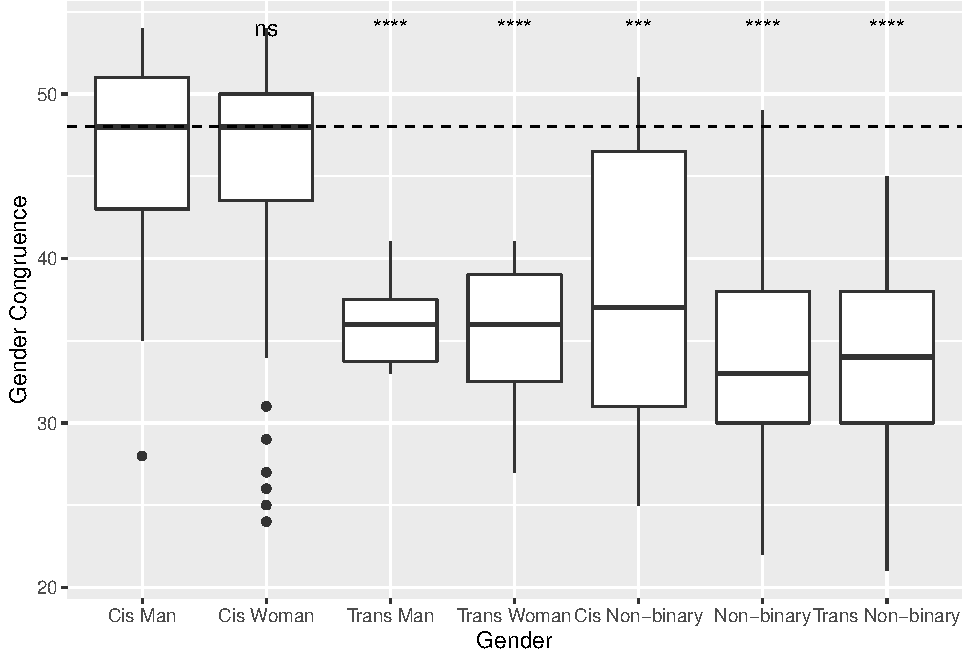
\includegraphics{thesis_files/figure-latex/congruence_graph-1.pdf}

\hypertarget{transgender-inclusive-behaviors}{%
\section{Transgender Inclusive Behaviors}\label{transgender-inclusive-behaviors}}

Kattari et al. (2018) developed the Transgender Inclusive Behavior Scale (TIBS) as a method of quantifying the number of behaviors that may support and include transgender people that one regularly does. Scores are a sum of responses on a series of five-point likert scales ranging from ``Never'' to ``Often.''

A single-sample t-test revealed that non-cisgender people (\emph{M} = 51.34, \emph{SD} = 9.14) reporting performing more inclusive behaviors than cisgender people (\emph{M} = 41.98, \emph{SD} = 9.26), \emph{t}(304.22) = 10.22, \emph{p} \textless{} 0.001.

A one-way ANOVA demonstrated that there was a significant effect of gender \emph{F}(6, 249) = 26.51, \emph{p} \textless{} 0.001.
A Tukey post-hoc comparison revealed that cisgender men (\emph{M} = 37.31, \emph{SD} = 8.92) do significantly fewer trans inclusive behaviors than cisgender women (\emph{M} = 44.43, \emph{SD} = 8.18), transgender men (\emph{M} = 55.91, \emph{SD} = 9.16), transgender women (\emph{M} = 50.58, \emph{SD} = 9.97), cisgender non-binary people (\emph{M} = 45.73, \emph{SD} = 8.18), non-binary people (\emph{M} = 49.26, \emph{SD} = 9.3), and transgender non-binary people (\emph{M} = 53.85, \emph{SD} = 7.71). Cisgender women do significantly fewer trans inclusive behaviors than transgender men, transgender women, non-binary people, and transgender non-binary people. Cisgender non-binary people also do fewer trans inclusive behaviors than transgender non-binary people.

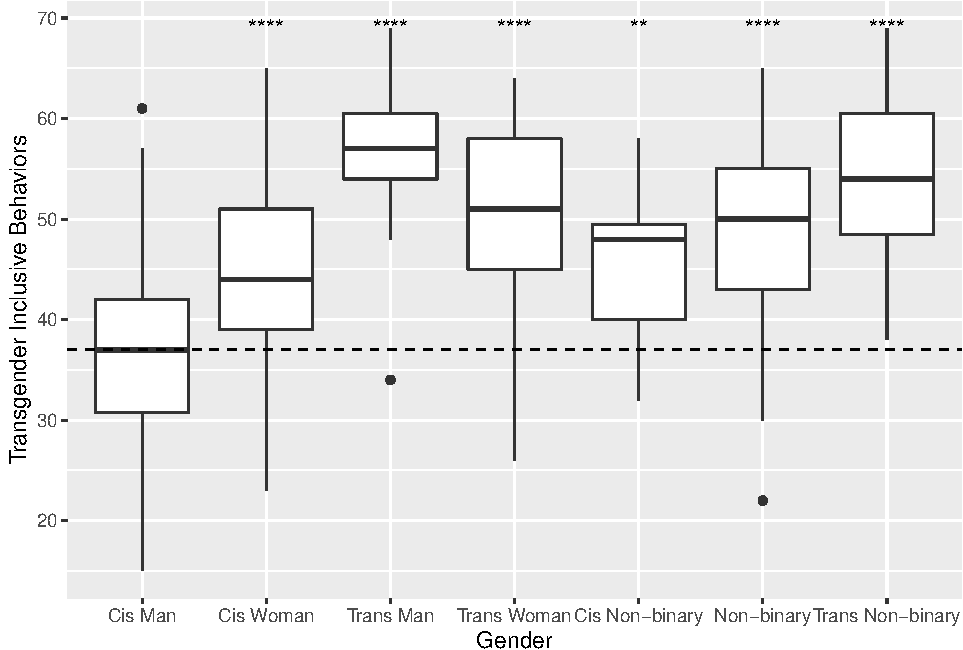
\includegraphics{thesis_files/figure-latex/incl_behavior_graph-1.pdf}

\hypertarget{pronouns-1}{%
\section{Pronouns}\label{pronouns-1}}

\hypertarget{comfort-sharing-pronouns}{%
\subsection{Comfort sharing pronouns}\label{comfort-sharing-pronouns}}

Items 1, 2, 3, 7, 8, and 9 touched upon participants desire to share their pronouns.

\hypertarget{desire-to-share-pronouns}{%
\subsection{Desire to share pronouns}\label{desire-to-share-pronouns}}

\hypertarget{concerns-about-sharing-pronouns}{%
\subsection{Concerns about sharing pronouns}\label{concerns-about-sharing-pronouns}}

\hypertarget{congruence-and-perception-of-pronouns}{%
\subsection{Congruence and perception of pronouns}\label{congruence-and-perception-of-pronouns}}

\hypertarget{historical-experience-at-reed-college}{%
\subsection{Historical experience at Reed College}\label{historical-experience-at-reed-college}}

\hypertarget{primary-component-analysis}{%
\subsection{Primary Component Analysis}\label{primary-component-analysis}}

Principal component analysis (PCA) was used on the pronoun and misgendering data. Using a Screen plot, we retained three components with an eigenvalue of 2.96, accounting for 54.29\% of the variance.

Item

Comp. 1 Loading

Comp. 2 Loading

Comp. 3 Loading

cis

{-0.11}

{0.01}

{-0.01}

trans

{0.06}

{-0.02}

{-0.04}

nonbinary

{0.10}

{-0.02}

{0.02}

gender\_bin

{0.51}

{-0.09}

{0.16}

pronoun\_bin

{0.29}

{0.07}

{0.15}

comfort\_general

{-0.22}

{-0.21}

{0.00}

comfort\_reed

{-0.10}

{-0.22}

{0.03}

comfort\_class

{-0.13}

{-0.20}

{0.00}

desire\_general

{-0.01}

{-0.43}

{-0.05}

desire\_reed

{0.07}

{-0.44}

{0.00}

desire\_class

{0.04}

{-0.42}

{0.00}

comfort\_withsimilargenders

{0.25}

{-0.21}

{-0.02}

comfort\_someoneelsefirst

{0.02}

{-0.15}

{-0.24}

comfort\_proffirst

{0.02}

{-0.18}

{-0.21}

attention\_general

{0.23}

{0.12}

{-0.43}

attention\_reed

{0.10}

{0.18}

{-0.55}

attention\_class

{0.14}

{0.13}

{-0.38}

gender\_perception\_consistent

{-0.36}

{-0.01}

{-0.17}

gender\_pronouns\_consistent

{-0.15}

{-0.19}

{-0.22}

pronouns\_represent

{-0.15}

{-0.21}

{-0.25}

willmisgender\_ifnopronouns

{0.25}

{-0.10}

{-0.03}

assume\_pronouns\_correctly

{-0.32}

{0.04}

{-0.05}

understand\_better

{0.18}

{-0.19}

{-0.03}

profs\_share

{-0.06}

{0.00}

{0.22}

students\_share

{-0.03}

{-0.04}

{0.08}

reed\_support

{-0.15}

{0.09}

{0.15}

\hypertarget{discussion}{%
\chapter{Discussion}\label{discussion}}

So, we found some gendered pronouns.

\appendix

\backmatter

\hypertarget{references}{%
\chapter*{References}\label{references}}
\addcontentsline{toc}{chapter}{References}

\markboth{References}{References}

\noindent

\setlength{\parindent}{-0.20in}
\setlength{\leftskip}{0.20in}
\setlength{\parskip}{8pt}

\hypertarget{refs}{}
\begin{cslreferences}
\leavevmode\hypertarget{ref-kattariDevelopmentValidationTransgender2018}{}%
Kattari, S. K., O'Connor, A. A., \& Kattari, L. (2018). Development and Validation of the Transgender Inclusive Behavior Scale (TIBS). \emph{Journal of Homosexuality}, \emph{65}(2), 181--196. \url{http://doi.org/10.1080/00918369.2017.1314160}

\leavevmode\hypertarget{ref-kozeeMeasuringTransgenderIndividuals2012}{}%
Kozee, H. B., Tylka, T. L., \& Bauerband, L. A. (2012). Measuring Transgender Individuals' Comfort With Gender Identity and Appearance: Development and Validation of the Transgender Congruence Scale. \emph{Psychology of Women Quarterly}, \emph{36}(2), 179--196. \url{http://doi.org/10.1177/0361684312442161}

\leavevmode\hypertarget{ref-mclemoreExperiencesMisgenderingIdentity2015}{}%
McLemore, K. A. (2015). Experiences with Misgendering: Identity Misclassification of Transgender Spectrum Individuals. \emph{Self and Identity}, \emph{14}(1), 51--74. \url{http://doi.org/10.1080/15298868.2014.950691}

\leavevmode\hypertarget{ref-nagoshiGenderDifferencesCorrelates2008}{}%
Nagoshi, J. L., Adams, K. A., Terrell, H. K., Hill, E. D., Brzuzy, S., \& Nagoshi, C. T. (2008). Gender Differences in Correlates of Homophobia and Transphobia. \emph{Sex Roles}, \emph{59}(7-8), 521--531. \url{http://doi.org/10.1007/s11199-008-9458-7}

\leavevmode\hypertarget{ref-tateIntegratingStudyTransgender2014}{}%
Tate, C. C., Youssef, C. P., \& Bettergarcia, J. N. (2014). Integrating the Study of Transgender Spectrum and Cisgender Experiences of Self-Categorization from a Personality Perspective. \emph{Review of General Psychology}, \emph{18}(4), 302--312. \url{http://doi.org/10.1037/gpr0000019}
\end{cslreferences}

% Index?

\end{document}
